\part{Introducción a la Metalurgia}


\section{Diferencia entre lo micro y macro}

Los conjuntos diseñados por ingenieros tienen una forma \textbf{geométrica} y un \textbf{material}. Ambas son propiedades macroscópicas. 

Sin embargo, lo que determina en gran parte las propiedades de una pieza es su \textbf{estructura} al nivel atómico (Å) y microscópico (micrómetros). Estas no son evidentes al ojo humano y se necesita de instrumentos y técnicas para poder detectar y caracterizar estas estructuras.

Un objetivo fundamental de la metalurgia física es tratar de relacionar los aspectos macroscópicos perceptibles con los aspectos microscópicos y submicroscópicos mediante métodos \textbf{netamente científicos}. La metalurgia física es una ciencia aplicada.

\section{Nociones de materiales}

\subsection{Grupos de Materiales}

\begin{description}
    \item[Metales] Materiales con enlaces metálicos
    \item[Polímeros] Sustancias inorgánicas con enlaces no metálicos
    \item[Polímeros] Matríz metálica, polimérica o cerámica con partículas o fibras poliméricas o cerámicas 
\end{description}


\subsection{Características de los metales}
Como clase de material, los metales son aquellos materiales cuyos átomos están unidos mediante un enlace metálico. Algunos materiales poseen enlaces no metálicos y son considerados metales porque su enlace metálico es el que prevalece, como es el caso para la mayoría de los metales estudiados.

\begin{itemize}
    \item Deformables plásticamente
    \item Fáciles de conformar y unir
    \item Alta tenacidad
    \item Alta resistencia mecánica
    \item Alta rigidez
    \item Bajo costo
    \item Alta conductividad eléctrica y térmica
    \item Fácilmente reciclables
    \item Baja resistencia a la corrosión
    \item Alta densidad
\end{itemize}



\subsection{Aleaciones metálicas}

Se define como un material compuesto por varias clases de átomos (metálicos y/o no metálicos) unidos mediante un enlace principalmente metálico.

El \textbf{elemento base} de la aleación es el elemento químico mayoritario y siempre es de carácter metálico. Los \textbf{aleantes} son elementos cuya presencia se debe a una adición \textit{intencional} durante el proceso de fabricación de la aleación. Cumplen funciones específicas. En general hay un \textbf{aleante principal} que le otorga las características principales a la aleación y no tiene porque ser el de mayor proporción.

Los átomos que no fueron agregados intencionalmente sino que provienen de alguna/s de las materias primas usadas para la fabricación de la aleación (mineral, fundente, combustible, oxidante) y no han podido ser totalmente eliminados en el proceso de fabricación se llaman \textbf{residuales}. Se pueden categorizar en dos clases

\begin{description}
    \item[Residuales no nocivos] No tienen efectos negativos de importancia y pueden hasta mejorar alguna propiedad
    \item[Residuales nocivos o impurezas] Influyen negativamente en algunas propiedades de importancia para la aleación. Su reducción conlleva con un aumento del costo.  
\end{description}

\section{Unión entre átomos}

\begin{figure}
    \centering
    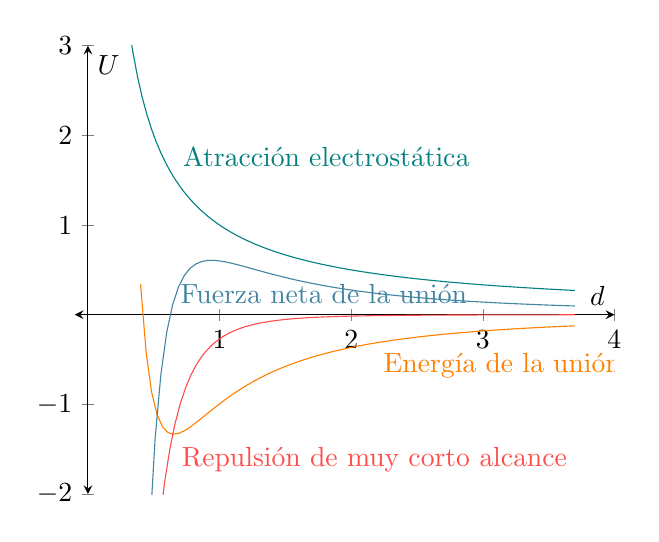
\begin{tikzpicture}[>=stealth]
    \begin{axis}[
        xmin=-.1,xmax=4,
        ymin=-2,ymax=3,
        axis x line=middle,
        axis y line=middle,
        axis line style=<->,
        xlabel={$d$},
        ylabel={$U$},
        cycle list name=exotic,no marks
        ]
        \addplot expression[domain=.2:3.7,samples=100]{1/x} 
                    node[pos=0.5,anchor=south west]{Atracción electrostática}; 
        \addplot expression[domain=.4:3.7,samples=80]{(x-2*(x+.04)^2)/((x+.04)^4)}  
        node[pos=.7,anchor=north west]{Energía de la unión};
        \addplot expression[domain=.2:3.7,samples=80]{-(x-1.6*x^2)/((x)^4)}  
        node[pos=.96,anchor=south west]{Fuerza neta de la unión};
        \addplot expression[domain=.5:3.7,samples=80]{-1/(x+.3)^5}  node[pos=.3,anchor=north west]{Repulsión de muy corto alcance};
    \end{axis}
\end{tikzpicture}
\caption{Fuerzas que intervienen en una unión iónica. El punto donde la fuerza neta cruza el eje $x$ se denomina la distancia de equilibrio $d_0$ y es la distancia nominal entre átomos en un material. Este punto coincide con el mínimo de energía de la unión.}
\end{figure}

\begin{itemize}
    \item El mínimo de energía ($U_0$) está relacionado con la temperatura de sublimación y fusión
    \item La pendiente de la curva de la fuerza neta sobre $d_0$ son proporcionales al módulo elástico del metal (se relaciona también con la curvatura de la energía sobre $d_0$ también)
    \item La asimetría de la curva de energía está relacionada con el coeficiente de dilatación del metal. Cuanto más empinada cerca de 0 y más chata alejándose de cero, más se dilata el material.
\end{itemize}



Al \textbf{aumentar} la energía de la unión, la distancia de equilibrio ($d_0$) disminuye (\textbf{disminuyendo la curvatura de la energía}), la curva de energía se vuelve \textbf{más simétrica}. En consecuencia puede decirse que, en términos generales, en los metales puros se cumple que a mayor punto de fusión es \textit{mayor} el módulo elástico y \textit{menor} el coeficiente de dilatación lineal.

\section{Estructura cristalina de metales}

En estado sólido los metales son cristalinos, es decir que los átomos ocupan posiciones ordenadas dentro de una estructura. Existen materiales metálicos sin ordenamiento en su estructura.

Existen materiales metálicos sin ordenamiento en su estructura (vidrios metálicos), pero son la excepción.

\begin{description}
    \item[Red cristalina] Red de puntos imaginarios que ocupan posiciones ordenadas en el espacio de modo que cada punto tiene idénticos alrededores
    \item[Motivo] Conjunto de átomos con una configuración determinada. Ocupa cada nodo de la red.
    \item[Estructura cristalina]  Red ordenada de puntos ubicándose en cada uno de ellos un mismo motivo constituido por átomos de metal
    \item[Parámetro de red] es la distancia entre átomos medida en las direcciones de los ejes principales de la celda de la red. Dependiendo de la configuración de la red (FCC/HCP/BCC) puede haber más de un parámetro. Suele ser del orden de unas décimas de nanómetro para metales.
\end{description}

\subsection{Características de estructuras cristalinas en metales}

\subsubsection{Estructura FCC}
Es una de las dos estructuras de máxima compacidad.
En general los FCC son metales de alta ductilidad y maleabilidad, baja tensión de fluencia, y alta tenacidad que además no presentan transición dúctil-frágil. 

\subsubsection{Estructura HCP}
Es una de las dos estructuras de máxima compacidad. Los HCP en general son metales menos dúctiles y más anisotrópicos que los FCC o BCC.


\subsubsection{Estructura BCC}
No posee planos de máxima compacidad. Los BCC poseen menor ductilidad y tenacidad que los FCC pero mayor tensión de fluencia. Presentan transición dúctil-frágil.

\subsection{Índices de Miller (incompleto)}

\subsection{Defectos cristalinos}

